\documentclass[
	% -- opções da classe memoir --
	article,			% indica que é um artigo acadêmico
	11pt,				% tamanho da fonte
	oneside,			% para impressão apenas no verso. Oposto a twoside
	a4paper,			% tamanho do papel. 
	% -- opções da classe abntex2 --
	%chapter=TITLE,		% títulos de capítulos convertidos em letras maiúsculas
	%section=TITLE,		% títulos de seções convertidos em letras maiúsculas
	%subsection=TITLE,	% títulos de subseções convertidos em letras maiúsculas
	%subsubsection=TITLE % títulos de subsubseções convertidos em letras maiúsculas
	% -- opções do pacote babel --
	english,			% idioma adicional para hifenização
	brazil,				% o último idioma é o principal do documento
	sumario=tradicional
]{abntex2}

% ---
% Pacotes fundamentais 
% ---
\usepackage{lmodern}			% Usa a fonte Latin Modern
\usepackage[T1]{fontenc}		% Selecao de codigos de fonte.
\usepackage[utf8]{inputenc}		% Codificacao do documento (conversão automática dos acentos)
\usepackage{indentfirst}		% Indenta o primeiro parágrafo de cada seção.
\usepackage{nomencl} 			% Lista de simbolos
\usepackage{color}				% Controle das cores
\usepackage{graphicx}			% Inclusão de gráficos
\usepackage{microtype} 			% Para melhorias de justificação

% ---
% Pacotes glossaries
% ---
\usepackage[subentrycounter,seeautonumberlist]{glossaries}
% ---

% ---
% Pacotes de citações
% ---
\usepackage[brazilian,hyperpageref]{backref}	 % Paginas com as citações na bibl
\usepackage[alf]{abntex2cite}	% Citações padrão ABNT
% ---

%Muda o contador para sections.
\usepackage{chngcntr}
\counterwithin{section}{chapter}


\titulo{Camada Lógica de Cache na Arquitetura Aplicações Móveis Multi Plataforma Baseada em Tecnologias Abertas}
\autor{Marcus Vinícius de Lima\thanks{\url{marcvlima@gmail.com}}}
\local{Brasil}

% ---
% Configurações de aparência do PDF final

% alterando o aspecto da cor azul
\definecolor{blue}{RGB}{41,5,195}

% informações do PDF
\makeatletter
\hypersetup{
	%pagebackref=true,
	pdftitle={\@title}, 
	pdfauthor={\@author},
	pdfsubject={Modelo de artigo científico com abnTeX2},
	pdfcreator={LaTeX with abnTeX2},
	pdfkeywords={abnt}{latex}{abntex}{abntex2}{atigo científico}, 
	colorlinks=true,       		% false: boxed links; true: colored links
	linkcolor=blue,          	% color of internal links
	citecolor=blue,        		% color of links to bibliography
	filecolor=magenta,      		% color of file links
	urlcolor=blue,
	bookmarksdepth=4
}
\makeatother
% --- 

% ---
% compila o indice
% ---
\makeindex
% ---

% ---
% entradas do glossario
% ---
 \newglossaryentry{sdk}{
 	name={SDK},
 	plural={SDKs},
 	description={Software Development Kit - Kit de Desenvolvimento de Software. Conjunto de ferramentas empregadas no processo de desenvolvimento de software}
}
\newglossaryentry{back-end}{
	name={Back-end},
	plural={Back-ends},
	description={Num sistema que emprega a arquitetura cliente servidor, o termo back end e empregado para referenciar o conjunto de camadas que constituem a parte servidor}
}

\newglossaryentry{add}{
	name={ADD},
	description={Attribute Drive Design - Método desenvolvido pelo SEI para realizar o desenho arquitetural através da decomposição iterativa do sistema e seus subcomponentes}
}

\makeglossaries
% ---
% Altera as margens padrões
% ---
\setlrmarginsandblock{3cm}{3cm}{*}
\setulmarginsandblock{3cm}{3cm}{*}
\checkandfixthelayout
% ---

% --- 
% Espaçamentos entre linhas e parágrafos 
% --- 

% O tamanho do parágrafo é dado por:
\setlength{\parindent}{1.3cm}

% Controle do espaçamento entre um parágrafo e outro:
\setlength{\parskip}{0.2cm}  % tente também \onelineskip

% Espaçamento simples
\SingleSpacing

% ---
% Exemplo de configurações do glossairo
\renewcommand*{\glsseeformat}[3][\seename]{\textit{#1}  
	\glsseelist{#2}}
% ---

\begin{document}
\graphicspath{images}	
\selectlanguage{brazil}
\maketitle

\selectlanguage{english}
\begin{abstract}
Abstract text.
\end{abstract}

\selectlanguage{brazil}

\begin{abstract}
Resumo em português.
\end{abstract}

\tableofcontents

\chapter{Introdução}
\section{Problema}
\section{Objetivos}
\chapter{Referencial Teórico}
\section{Arquitetura de Software}

Segundo \cite{bass2012practice} a arquitetura de software é um conjunto de estruturas necessárias para permitir racionalizar sobre um sistema, que compreende desde elementos de software os relacionamentos entre estes e propriedades definidas sobre ambos.

Martin Fowler com sua visão pragmática em \cite{fowler2002patterns} cita alguns pontos recorrentes que definem arquitetura de software:
\begin{enumerate}
	\item O mais elevado nível de separação do sistema em suas partes.
	\item As decisões que são mais difíceis de serem alteradas.
	\item Existem múltiplas arquiteturas em um sistema.
	\item O que é arquiteturalmente significativo pode mudar ao longo do ciclo de vida do projeto.
	\item Arquitetura se resume a tudo o que é importante.
\end{enumerate}




\section{Aplicações Móveis Multiplataforma}
Recentemente as aplicações móveis tem apresentado um crescimento expressivo. Desde a queda de popularidade das plataformas mobile BlackBerry, Bada e Symbian, iOS e Android tem adquirido uma força expressiva no mercado \cite{dalmasso2013survey}.

Porém, a diversidade das plataformas e a variedade de \gls{sdk} e ferramentas disponíveis criou uma segmentação desafiadora para o mercado de desenvolvimento de aplicações móveis \cite{dalmasso2013survey}.

A grande maioria dos desenvolvedores e organizações querem atingir a maior fatia de mercado com seus aplicativos. Para tal é necessário que o aplicativo esteja disponível nas principais plataformas mobile como o iOS, Android e Windows Phone. 

Porém o desenvolvimento para estas plataformas requerem amplo conhecimento do desenvolvedor sobre as mesmas e sobre os seus respectivos \gls{sdk}, o que eleva o custo de desenvolvimento e a complexidade do processo. Para contrapor a esta barreira imposta pela pluralidade de plataformas de desenvolvimento móvel, entra em cena a abordagem multiplataforma, capaz de reduzir o esforço de desenvolvimento e o tempo para lançamento de aplicativos no mercado \cite{dalmasso2013survey}.

Como citado em \cite{shehab2014reducing} a vantagem de custo e tempo de mercado proporcionado por esta abordagem está promovendo o surgimento de distintas plataformas que a adotam. Essas plataformas estão competindo pela adoção de desenvolvedores em características como o número de plataformas nativas suportadas, acesso a funções nativas dos dispositivos móveis, facilidade de acesso ao \gls{back-end} e por melhorias de performance. 

\section{Cache de Aplicações Móveis}

O paradigma cliente-servidor para aplicações móveis apresenta peculiaridades significativas quando comparado as aplicações tradicionais, provocadas sobretudo por dois fatores: perda de conectividade frequente e baixa largura de banda dos dispositivos móveis \cite{rathore2007overview}.
Tais fatores geram a necessidade de que seja reduzida a comunicação cliente servidor, tornando o mecanismo de cache uma solução amplamente desejável \cite{rathore2007overview}.

A otimização do tempo de resposta do ponto de vista do usuário de aplicações móveis é apresentada em \cite{xing2015user} também como justificativa para o mecanismo de cache.
 
 Em \cite{rathore2007overview} os mecanismos de cache são caracterizados por 3 componentes: granularidade de caching, estratégia de coerência de cache e política de substituição de cache.

\subsection{Granularidade de Cache}
Granularidade de caching diz respeito a escolha do tipo correto de informação que deve ser mantido em cache para permitir a correta utilização do armazenamento do dispositivo.

\subsection{Estratégia de Coerência de Caching}
Uma vez definido que informações devem ser mantidas em cache, o próximo passo é definir a estratégia de coerência de cache, que consiste em manter as informações do cache consistentes com os dados do servidor..

\begin{enumerate}
	\item Invalidação temporal-dependente:  Quando algum item é alterado no servidor.
	\item Invalidação dependente de localização: Quando a mudança de localização do cliente provoca a invalidação do item.
\end{enumerate}

\subsection{Política de Substituição de Caching}
Após serem identificados os itens de cache inválidos, a politica de substituição de cache define como a informação armazenada no cliente deverá ser atualizada quando é atingido um limite local de armazenamento.

Um dos mecanismos mais comumente utilizados para substituição de cache é o algoritmo de LRU \emph{Least Recent User}, onde o item com maior tempo sem ser utilizado pela aplicação é substituído \cite{xing2015user}.

\section{Condutores Arquiteturais para uma Aplicação Móvel}
Um dos grandes fatores para garantia de qualidade no desenvolvimento de aplicações consiste na correta identificação de seus condutores arquiteturais e os mecanismos que irão assegurar uma implementação que os atenda \cite{bachmann2001introduction}.

Condutores arquiteturais são o uma combinação de requisitos funcionais, requisitos de qualidade e restrições que influenciam na determinação das características arquiteturais da aplicação \cite{bachmann2001introduction}.

No contexto de aplicações móveis os seguintes requisitos arquiteturais são elencados:
\begin{enumerate}
	\item Suporte para conexões instáveis \cite{tiffany2008guide}: A aplicação deve estar preparada para eventuais falhas de conectividade.
	
	\item Suporte para baixa largura de conexão \cite{tiffany2008guide}: Uma aplicação móvel deve estar preparada para assegurar que as operações sejam realizadas mesmo em cenários de baixa largura de banda.
	
	\item Suporte para velocidades de \emph{upstream} reduzidas \cite{rathore2007overview}: As requisições de uma aplicação móvel para o servidor devem ser otimizadas para conter a menor quantidade de dados possível.
	
	\item Otimização de bateria \cite{rathore2007overview}: Uma aplicação móvel deve ser projetada de modo a consumir a menor quantidade de energia possível.
	
	\item Espaço de armazenamento reduzido \cite{tiffany2008guide}: Uma aplicação deve otimizar a quantidade de dados que é armazenada para o seu funcionamento.
	
\end{enumerate}

Como este trabalho tem por objetivo a elaboração de uma arquitetura genérica apenas os condutores arquiteturais mais importantes de uma aplicação móvel estão sendo considerados. Ao considerar uma aplicação específica, os requisitos arquiteturais devem ser definidos de maneira mais detalhada. Uma das metodologias que poderia ser empregada para definição de requisitos arquiteturais, está definida em \cite{eeles2005capturing}.

\section{Separação de Responsabilidades da Aplicação em Camadas Lógicas}

Conforme descrito em \cite{griss1998architecting} aplicações e componentes que que interagem entre sí utilizando uma arquitetura modular e baseada em camadas garantem estruturas e mecanismos consistentes.

A separação de responsabilidades favorece a otimização de componentes, uma vez que a sua refatoração pode ser realizada sem afetar componentes adjacentes. Essa abordagem torna uma aplicação mais compreensível e facilita a manutenção de sistemas interdependentes \cite{meier2009microsoft}.

Uma arquitetura baseada em camadas favorece a separação de responsabilidades. Cada tipo de tarefa que deve ser realizado no contexto da aplicação deve ser organizado em grupos de tarefas relacionadas. Esse grupo dará origem a uma camada lógica que realizam tarefas com um propósito semelhante \cite{meier2009microsoft}. 

Independentemente se será empregada uma abordagem de camada mais estrita onde uma camada pode se comunicar imediatamente com camada adjacente, ou se pode ser considerada uma arquitetura mais flexível onde a comunicação entre camadas não adjacentes é permitida, deve ser favorecida sempre uma abstração no estabelecimento da comunicação. Tal abstração garantida através do estabelecimento de uma interface de comunicação entre camadas assegura a manutenção da alta coesão e do baixo acoplamento na arquitetura dos sistema \cite{meier2009microsoft}.

\chapter{Metodologia}
Este trabalho foi desenvolvimento considerando as seguinte etapas:

\begin{enumerate}
	
	\item Realizar revisão bibliográfica sobre aplicações móveis multiplataforma sua motivação e características.
	
	\item Realizar revisão bibliográfica sobre os princípios e técnicas de cache de aplicações móveis.
	
	\item Identificar na literatura os condutores arquiteturais que devem ser considerados na definição de uma arquitetura de cache de aplicações móveis.
	
	\item Definir os componentes básicos de uma arquitetura que atenda aos condutores arquiteturais propostos.
	
	\item Definir de maneira detalhada os papeis e associações entre os componentes e mecanismos arquiteturais segundo preceitos da recomendação IEEE Standard 1471-2000 além das práticas de descrição arquitetural definidas em \cite{bass2012practice}\cite{bachmann2010DocumentingSoftware}.
	
	\item Empregar a metodologia ATAM para avaliar a consonância da arquitetura proposta para atender aos condutores arquiteturais considerados.
\end{enumerate}

\section{Arquitetura Proposta}
A proposta apresentada por este trabalho consiste em aplicar uma arquitetura baseada em camadas para solucionar o problema associado ao tratamento de cache em aplicações móveis multiplataforma.

Este estilo arquitetural permite abstrair todas as funcionalidades relacionadas ao tratamento de cache de maneira modular separando as responsabilidades e elevando o nível de flexibilidade e manutenabilidade da solução.

\begin{figure}
	\centering
	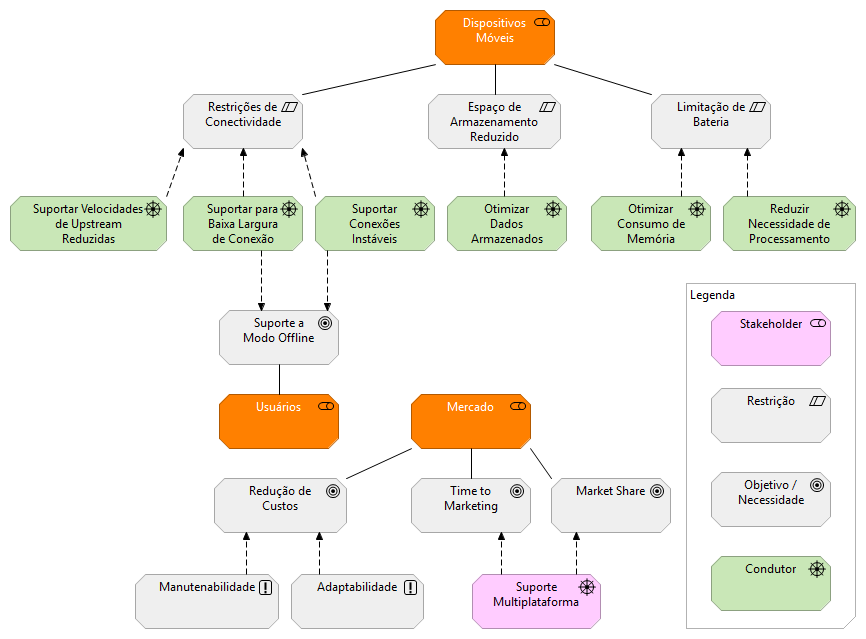
\includegraphics[scale=0.5]{images/UtilityTree}
	\caption{Árvore de Utilidade Adaptada: Stakeholders, Restrições, Objetivos, Necessidades, Condutores e suas Relações}
\end{figure}


Aplicando o método \gls{add} no passo inicial a arquitetura geral será descrita através da exposição de suas camadas mais granulares e suas responsabilidades.

\begin{figure}
	\centering
	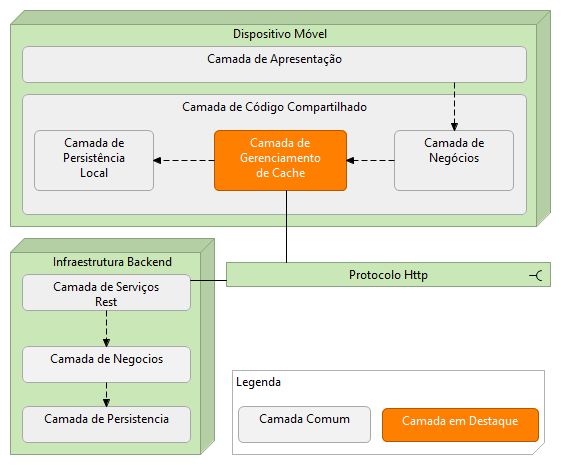
\includegraphics[scale=0.7]{images/CamadasNivel0}
	\caption{Camada de Gerênciamento de Cache e suas Interações}
\end{figure}

\begin{description}
	\item Camada de Apresentação:
	Localizada no dispositivo móvel e sua principal responsabilidade é permitir a interação entre o usuário e a aplicação.
	Numa aplicação móvel multiplataforma a camada de apresentação pode ser uniforme entre diferentes plataformas ou ser customizada para cada plataforma em que o sistema terá suporte.
	\item Camada de Código Compartilhado:
	Também localizada no dispositivo móvel constitui o coração da abordagem multiplataforma. Esta camada é responsável por agregar todos os componentes da aplicação que deverão serem compartilhados entre todas as plataformas suportadas empregando o mesmo code-base, para garantir consistência e reutilização de código.
	\begin{description}
		\item Camada de Negócios:
		Contida no dispositivo móvel é responsável por concentrar as regras de negócios da aplicação intimamente relacionadas a apresentação, incluindo formatação exibição e resposta imediata para estímulos provenientes da interação do usuário.
		\item Camada de Persistência Local: 
		Presente no dispositivo móvel é responsável realizar e gerenciar o acesso aos mecanismos de persistência local da aplicação.
		\item Camada de Gerenciamento de Cache:
		Inserida no dispositivo móvel é o segmento principal da proposição arquitetural deste trabalho. Sua atribuição é gerenciar o cache local da aplicação onde devem ser implementados todos os mecanismos de granularidade, coerência e política de substituição de cache.
	\end{description}
	\item Camada de Serviços Rest:
	Contida no \gls{back-end} é responsável por fornecer uma fachada com os serviços que podem ser consumidos pelo cliente local.
	\item Camada de Negócios:
	Também contida no \gls{back-end} é responsável por implementar todas as regras de negócio da aplicação bem como interagir com demais sistemas que fazem fronteira com a aplicação móvel, como por exemplo sistemas legados ou outros serviços internos da organização ou mesmo serviços de terceiros.
	\item Camada de persistência:
	Localizada na infraestrutura \gls{back-end} é responsável por gerenciar e implementar o armazenamento persistente dos dados da aplicação.
\end{description}

Na arquitetura proposta a Camada de Gerenciamento de Cache possui fronteira com três outras camadas possuindo um papel de destaque arquitetural por ser um elo chave entre os elementos do sistema e especialmente por conectar o segmento cliente ao segmento \gls{back-end} da aplicação.
 

\subsection{Importancia de Tecnologias Abertas}

\subsection{Apache Cordova}

\subsection{SQLite}

\subsection{AngularJS}

\subsection{Prova de Conceito da Arquitetura Proposta}

\chapter[ChaConclusao]{Conclusão}

\section{Trabalhos Futuros}

\bibliography{artigo}{}

% ----------------------------------------------------------
% Glossário
% ----------------------------------------------------------

% ---
% Define nome e preâmbulo do glossário
% ---
\renewcommand{\glossaryname}{Glossário}
%\renewcommand{\glossarypreamble}{Esta é a descrição do glossário.\\ \\}

% ---
% Traduções para o ambiente glossaries
% ---
\providetranslation{Glossary}{Glossário}
\providetranslation{Acronyms}{Siglas}
\providetranslation{Notation (glossaries)}{Notação}
\providetranslation{Description (glossaries)}{Descrição}
\providetranslation{Symbol (glossaries)}{Símbolo}
\providetranslation{Page List (glossaries)}{Lista de Páginas}
\providetranslation{Symbols (glossaries)}{Símbolos}
\providetranslation{Numbers (glossaries)}{Números} 
% ---

% ---
% Imprime o glossário
% ---
\cleardoublepage
\phantomsection
\addcontentsline{toc}{chapter}{\glossaryname}
% \glossarystyle{index}
% \glossarystyle{altlisthypergroup}
\glossarystyle{tree}
\printglossaries
% ---
% ---

\end{document}